\chapter{Locality and Caches}
\label{chap:locality}

\section{Locality of Reference}

\begin{definition}[Temporal locality]
  Accessing data that was accessed recently.
\end{definition}

\begin{definition}[Spatial locality]
  Accesing data close to data that was accessed recently.
\end{definition}

\section{Memory Hierarchies}

\begin{definition}[Cache]
  A smaller and faster memory that stores a subset of the contents of
  a larger and slower memory.
\end{definition}

\begin{figure}
  \centering

  \begin{center}
    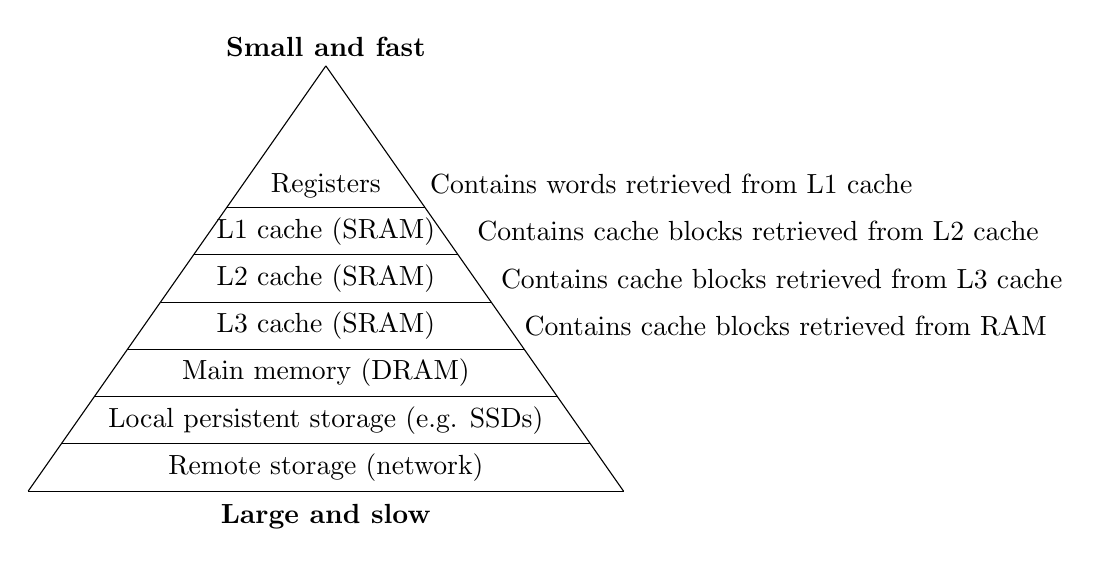
\begin{tikzpicture}[scale=0.6]
      \def \h {9};
      \def \f {.7};

      \foreach \y in  {0,1,2,3,4,5,6} {
        \def \w { \h*\f-\y*\f };
        \def \v { \y*\f-\h*\f };
        \draw (\v,\y) -- (\w,\y);
      }

      \draw (-\h*\f,0)  -- (0,\h);
      \draw (\h*\f,0)  -- (0,\h);

      \node at (0,0) [above] {Remote storage (network)};
      \node at (0,1) [above] {Local persistent storage (e.g. SSDs)};
      \node at (0,2) [above] {Main memory (DRAM)};
      \node at (0,3) [above] {L3 cache (SRAM)};
      \node[align=left] at (4,3.5) [right] {Contains cache blocks retrieved from RAM};
      \node at (0,4) [above] {L2 cache (SRAM)};
      \node[align=left] at (3.5,4.5) [right] {Contains cache blocks retrieved from L3 cache};
      \node at (0,5) [above] {L1 cache (SRAM)};
      \node[align=left] at (3,5.5) [right] {Contains cache blocks retrieved from L2 cache};
      \node at (0,6) [above] {Registers};
      \node at (2,6.5) [right] {Contains words retrieved from L1 cache};

      \node at (0,9) [above] {\textbf{Small and fast}};
      \node at (0,-1) [above] {\textbf{Large and slow}};
    \end{tikzpicture}
  \end{center}

  \caption{Example memory hierarchy.}
  \label{fig:memory-hierarchy}
\end{figure}

\begin{definition}[Cache block]
  A $B$-byte chunk of memory, where $B$ is a power of two.
\end{definition}

\begin{definition}[Cache line]
  A structure that contains a cache block as well as metadata about
  the origin of the block.
\end{definition}

\begin{definition}[Cache hit]
  A memory operation to an address that is present in the cache.
\end{definition}

\begin{definition}[Cache miss]
  A memory operation to an address that is not present in the cache.
\end{definition}

\begin{definition}[Program working set]
  The amount of memory accessed by the program.
\end{definition}

\begin{definition}[Compulsory miss]
  A miss that occurs because the cache is empty.
\end{definition}

\begin{definition}[Conflict miss]
  A miss that occurs because too many blocks of the program working
  set are mapped to the same cache set.
\end{definition}

\begin{definition}[Capacity miss]
  A miss that occurs because the program working set exceeds the cache
  capacity.
\end{definition}

\section{Cache Organisation}

\section{Cache Performance}

%%% Local Variables:
%%% mode: latex
%%% TeX-master: "notes"
%%% End:
